\chapter{Systembeskrivelse}
Systemet, der er blevet udviklet er en blodtryksmåler. Blodtryksmåleren er tiltænkt at fungere som en invasiv blodtryksmåler på operationsstuer, der skal monitorerer patienters blodtryks under operationer.\\

\begin{figure}[H]
	\centering
	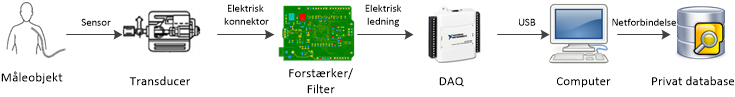
\includegraphics[width=1\textwidth]{Figurer/Systembeskrivelse}
	\caption{Forsøgsopstilling grafisk}
	\label{opstilling}
\end{figure} 
For at kunne lave et sådan system er der blevet udviklet en hardware del og en software del. 
Hardware delen er bestående af en forstærker, og et filter. Forstærkeren forstærker signalet til et håndterbart område, som arbejder sammen med en AD-konverter. Desuden består systemet også af et analogt lavpas filter, som filtrerer 50 Hz støj fra signalet. Hele systemet er koblet til en transducer, som dernæst er koblet intravenøst til borgeren. Transduceren giver systemet trykændrings feedback i enheden milivolt.  \\ [1ex]

Software delen bestående af en brugergrænseflade samt program med tilhørende database. Brugergrænsefladen viser et digitalt signal via programmet samt giver mulighed for forskellige funktioner og oplysninger. Yderligere består programmet af en mulighed for en digital filtrering af blodtrykssignalet samt algortimer til detektering af systole, diastole og puls. Systemet kan desuden lagre data fra signalet i en privat database.\\[1ex]

Hardwaren indhenter som nævnt signalet via en elektrisk konnnektor fra en transducer, som via en sensor henter et blodtryk intravenøst fra en eventuel patient. Yderligere, som figur \ref{opstilling} viser, er filteret/forstærkeren forbundet med en DAQ, som modtager det nu forstærkede og filtrerede signal. Til slut sendes signalet fra DAQ via USB til en computer, hvor signalet vises.\\[1ex]
Projektets endelig produkt er en prototype af et blodtryksmålings system som kan benyttes til invasiv blodtryksmåling.


